\subsection{Three samples}
For testing 3 samples in ideal solution, we consider the following possibilities:

\begin{itemize}
  \item For all the samples negative. The probability is $(1-p)^3$. Only 1 test is required.
  \item For 1 of the samples positive, 2 of the samples negative. The probability is $p(1-p)^2$. 4 tests is required. But if the first 2 samples are tested negative, only 3 test is required as the last sample must be positive.
  \item For all the samples positive. The probability is $p^3$. 4 tests is required.
  \item For 2 of the samples positive, 1 negative. The probability is $p^2(1-p)$.  4 tests is required.
\end{itemize}
The expected number of test:
\\
\begin{displaymath}
t(p)=4p^{3}+1(1-p)^{3}+4p^{2}(1-p) \times 3+4p(1-p)^{2} \times 2+3p(1-p)^{2}
\end{displaymath}
\\
Simplifying $t(p)$, we get:
\\
\begin{displaymath}
t(p)=2p^{3}-7p^{2}+8p+1
\end{displaymath}
\\
For solving $t(p)=3$:

\begin{center}
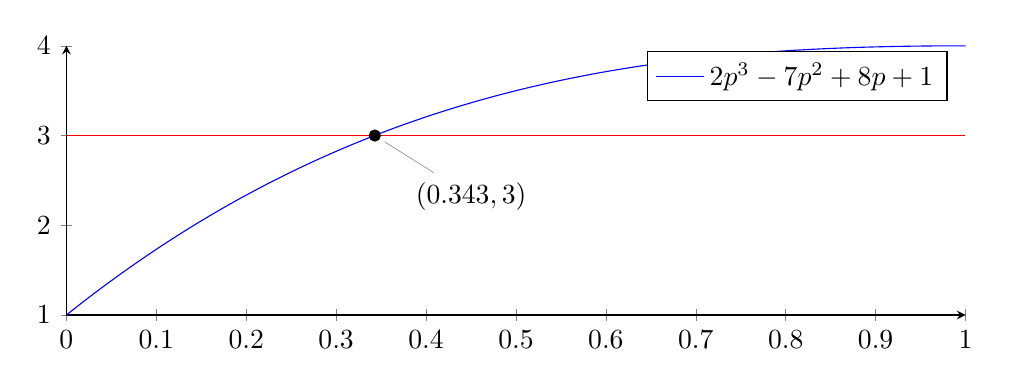
\begin{tikzpicture}
\begin{axis}[
    axis lines = left,
    ytick={0,1,2,3,4},
    xtick={0,0.1,0.2,0.3,0.4,0.5,0.6,0.7,0.8,0.9,1},
    height=5cm,
    width=13cm,
]

\addplot [
    domain=0:1, 
    samples=1000, 
    color=blue,
    ]
    {2*x^3 - 7*x^2 + 8*x + 1};
\addlegendentry{\(2p^{3}-7p^{2}+8p+1\)}

\addplot [
    domain=0:1, 
    samples=100, 
    color=red,
    ]
    {3};
    
\addplot[mark=*] coordinates {(0.343,3)} node[pin=310:{$(0.343,3)$}]{} ;

\end{axis}
\end{tikzpicture}
\end{center}
\\
From the graph, we find that when the group size is equal to 3, pooling should be used only when $p<0.343$ such that the expected amount of tests used is lower than the traditional way.
